% Generated by pq-experiments from measured benchmark records; no fitted data.
% Source data: source.csv and source.json.
% Requires: \usepackage{pgfplots} and \pgfplotsset{compat=1.18}.
\definecolor{pqR1CS}{HTML}{0072B2}
\definecolor{pqPlonkish}{HTML}{D55E00}
\definecolor{pqGreen}{HTML}{009E73}
\definecolor{pqPurple}{HTML}{CC79A7}
\definecolor{pqGold}{HTML}{E69F00}
\definecolor{pqIdeal}{HTML}{6B7280}
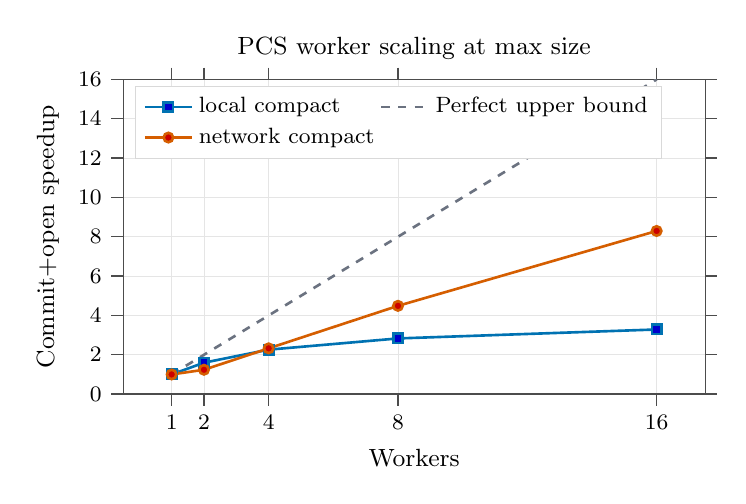
\begin{tikzpicture}
\begin{axis}[
  width=0.74\linewidth,
  height=0.46\linewidth,
  title={PCS worker scaling at max size},
  xlabel={Workers},
  ylabel={Commit+open speedup},
  axis background/.style={fill=white},
  grid=major,
  major grid style={draw=black!10, line width=0.25pt},
  axis line style={black!70, line width=0.45pt},
  tick align=outside,
  tick style={black!70, line width=0.45pt},
  tick label style={font=\footnotesize},
  label style={font=\small},
  title style={font=\small, yshift=-0.5ex},
  legend cell align={left},
  legend columns=2,
  transpose legend,
  legend style={at={(0.02,0.98)}, anchor=north west, draw=black!15, line width=0.25pt, fill=white, text opacity=1, font=\footnotesize},
  every axis plot/.append style={line width=0.95pt, mark options={scale=0.85, solid}},
  scaled ticks=false,
  unbounded coords=discard,
  xtick={1,2,4,8,16},
  ymin=0,
  ymax=16,
  ytick={0,2,4,6,8,10,12,14,16},
]
\addplot+[pqR1CS, solid, mark=square*] coordinates {(1, 1) (2, 1.598332) (4, 2.260581) (8, 2.831441) (16, 3.286933)};
\addlegendentry{local compact}
\addplot+[pqPlonkish, solid, mark=*] coordinates {(1, 1) (2, 1.239239) (4, 2.326973) (8, 4.488268) (16, 8.295907)};
\addlegendentry{network compact}
\addplot+[pqIdeal, dashed, mark=none] coordinates {(1, 1) (2, 2) (4, 4) (8, 8) (16, 16)};
\addlegendentry{Perfect upper bound}
\end{axis}
\end{tikzpicture}
